\chapter{Implementacija i korisničko sučelje}

    \section{Korištene tehnologije i alati}

    Koristili smo open-source sustav za upravljanje i pohranjivanje izvornog koda na platformi \textbf{GitLab}. \textit{( https://git-scm.com , https://gitlab.com )} \newline
    
    UML dijagrami izrađeni su uz pomoć \textbf{Astah Professional} aplikacije, a dijagrami baze podataka preko \textbf{ERDPlus}. \textit{( https://astah.net/products/astah-professional/ , https://erdplus.com/ )} \newline 
    
    Za komunikaciju s asistentom korišten je \textbf{Microsoft Teams}, a za međusobnu komunikaciju \textbf{WhatsApp}. Popis i podjela zadataka napravljena je na \textbf{Google Sheets}. \textit{( https://www.microsoft.com/hr-hr/microsoft-teams/group-chat-software/ , https://web.whatsapp.com/ , https://www.google.com/sheets/about/ )} \newline

    Za izradu dokumentacije primarno su korišteni \textbf{Overleaf} i \textbf{TeXstudio}. \textit{( https://www.overleaf.com , https://www.texstudio.org )} \newline
    
    Za pisanje frontend dijela aplikacije korištena je JavaScript biblioteka \textbf{React} te sintaksna ekstenzija JSX. Kod smo pisali u \textbf{Visual Studio Code-u}. Za kartu je korišten \textbf{Mapbox API}. \textit{( https://code.visualstudio.com , https://www.mapbox.com , https://www.npmjs.com , https://reactjs.org )} \newline
    
    Backend dio aplikacije pisan je u \textbf{Intellij IDEA} IDE-u u radnom okviru \textbf{Spring Boot} jezikom Java. \textit{( https://www.jetbrains.com/idea/ )} \newline

    Za deploy baze podataka (kao i aplikacije) korišten je \textbf{DigitalOcean}, a ista baza podataka korištena je i za testiranja. \textit{( https://www.digitalocean.com/ )}

    \section{Ispitivanje programskog rješenja}

    U nastavku ovog poglavlja biti će opisano ispitivanje implementiranih funkcionalnosti na razini komponenti te na razini cijelog sustava s prikazom odabranih ispitnih slučajeva.\newline
    
    U ispitivanju sustava korišten je radni okvir \textit{Selenium} te programsko sučelje \textit{Selenium WebDriver}. Metoda koja slijedi poziva se prije izvršavanja svakog testa.

    \begin{lstlisting}[language=Java,breaklines=true]
    @BeforeEach
	public void init() {
	   driver = new ChromeDriver();
	   System.setProperty("webdriver.chrome.driver", "C:\\Program Files (x86)\\Chrome Driver\\chromedriver.exe");
    
    driver.manage().timeouts().implicitlyWait(Duration.ofSeconds(10));
	   driver.get("http://dog-friendly.me/");
	}
    \end{lstlisting}

    \subsection{Ispitivanje komponenti}
    
    U prvom testu stvaramo objekt korisnika s već postojećim podatcima. Pozivamo funkciju koja se poziva prilikom pokušaja registracije. Test je uspješan ako test vrati vrijednost \textit{true} koja nam govori da korisnik s tom mail adresom već postoji.

    \begin{lstlisting}[language=Java,breaklines=true]
    @Test
    @Order(1)
    public void testCreateExistingUserException() {
        Account user = new Account(71l, "lm53309@fer.hr", "Husky123",
                "Novi dućan", UserRole.BUSINESS, false, false);

        accountService.existsByEmail(user.getEmail());

        assertEquals(true, accountService.existsByEmail(user.getEmail()));
    }
    \end{lstlisting}

    \eject
    Drugi test provjerava funkciju promjene podataka lokacije. Želimo promijeniti samo jedan podatak (u ovom slučaju opis) dok ostali podatci moraju ostati isti. Test je Uspješan ako je objekt nakon promjene jednak spremljenoj lokaciji s novim podatkom.

    \begin{lstlisting}[language=Java, breaklines=true]
    @Test
    @Order(2)
    public void testLocationChange() {
        LocationChangeRequest locationChangeRequest = new LocationChangeRequest(2l, null,
                null, "Fakultet elektrotehnike i računarstva", null, null);
        LocationResponse locationResponse = locationService.getByLocationId(locationChangeRequest.getLocationId());
        Location location = new Location(
                locationResponse.getLocationId(),
                locationResponse.getLongitude(),
                locationResponse.getLatitude(),
                locationResponse.getAddress(),
                locationChangeRequest.getLocationName() != null ? locationChangeRequest.getLocationName() : locationResponse.getLocationName(),
                locationChangeRequest.getLocationDescription() != null ? locationChangeRequest.getLocationDescription() : locationResponse.getLocationDescription(),
                locationChangeRequest.getPromoted() != null ? locationChangeRequest.getPromoted() : locationResponse.getPromoted(),
                locationChangeRequest.getDogFriendly() != null ? locationChangeRequest.getDogFriendly() : locationResponse.getDogFriendly(),
                accountService.findByAccountId(71l),
                locationTypeService.findByLocationTypeId(locationChangeRequest.getLocationTypeId() != null ? locationChangeRequest.getLocationTypeId() : locationResponse.getLocationTypeId()).orElse(null)
        );

        locationService.save(location);

        assertEquals(location, locationService.save(location));
    }
    \end{lstlisting}

    \eject
    Treći test radi provjeru funkcije za pretraživanje. Navodimo string lokacije koja postoji u sustavu. Test je uspješan ako je lokacija nađena funkcijom jednaka stringu.

    \begin{lstlisting}[language=Java, breaklines=true]
    @Test
    @Order(3)
    public void testSearchLocation() {
        String description = "808";
        List<LocationResponse> locations = locationService.search(description);
        LocationResponse location = locations.get(0);

        assertEquals("808", location.getLocationName());
    }
    \end{lstlisting}

    Četvrtim testom pokušavamo dohvatiti srednju vrijednost recenzije za lokaciju određenu s \textit{locationId}. Test je uspješan ako je dohvaćena vrijednost jednaka očekivanoj.

    \begin{lstlisting}[language=Java, breaklines=true]
    @Test
    @Order(4)
    public void testReviewAverage() {
        Long locationId = 2l;
        reviewService.getAverageForLocation(locationId);
        double avrg = (double) 13/3;

        assertEquals(Double.valueOf(avrg), reviewService.getAverageForLocation(locationId));
    }
    \end{lstlisting}

    Peti test provjerava funkciju za autentifikaciju korisnika. Korisnik se pokušava ulogirati na račun, ali s pogrešnom lozinkom. Ovaj test je uspješan ako kao odgovor dobijemo HttpStatus.BADREQUEST.

    \begin{lstlisting}[language=Java, breaklines=true]
    @Test
    @Order(5)
    public void testIncorrectPassword() {
        String email = "lm53309@fer.hr";
        String password = "provala";

        Authentication authentication;
        ResponseEntity responseEntity = new ResponseEntity(HttpStatus.OK);

        try {
            authentication = authenticationManager.authenticate(
                    new UsernamePasswordAuthenticationToken(email, password));
        } catch(BadCredentialsException e) {
            responseEntity = new ResponseEntity<>(HttpStatus.BAD_REQUEST);
        }

        assertEquals(HttpStatus.BAD_REQUEST, responseEntity.getStatusCode());
    }
    \end{lstlisting}

    U posljednjem testu provjeravamo povezanost lokacije s korisnikom koji ju je kreirao. Korisnik pokušava promijeniti lokaciju koju on nije kreirao. Prilikom promjene prvo se provjerava ima li korisnik ovlasti za odabranu akciju. Test je uspješan ako kao odgovor dobijemo da korisnik nema dozvolu za promjenu (HttpStatus.UNAUTHORIZED).

    \begin{lstlisting}[language=Java, breaklines=true]
    @Test
    @Order(6)
    public void testUnauthorizedLocationChange() {
        Long currentlyLoggedInAccountId = 71l;
        Long locationId = 196l;
        LocationResponse locationResponse = locationService.getByLocationId(locationId);
        ResponseEntity responseEntity = new ResponseEntity(HttpStatus.OK);

        if(locationResponse.getAccountId() != currentlyLoggedInAccountId)
            responseEntity = new ResponseEntity<>(HttpStatus.UNAUTHORIZED);

        assertEquals(HttpStatus.UNAUTHORIZED, responseEntity.getStatusCode());
    }
    \end{lstlisting}

    \eject
    \textbf{Svi ispitani testovi su bili uspješni}

    \begin{figure}[H]
        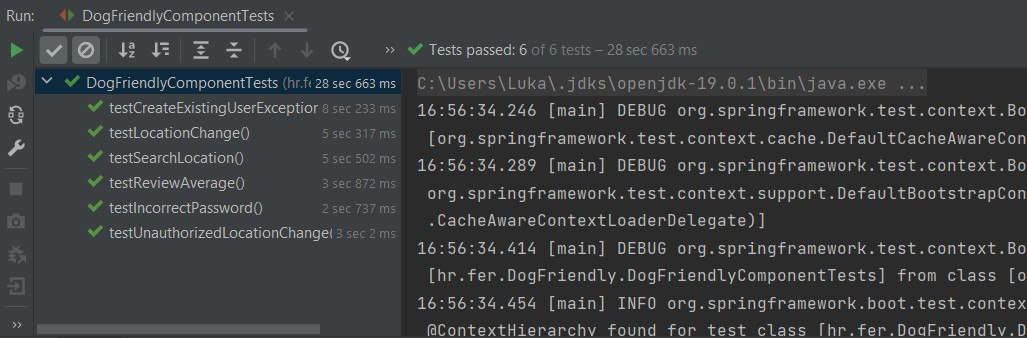
\includegraphics[width=\textwidth]{img/Ispitivanje komponentni.jpg}
        \centering
        \caption{Rezultati testova ispitivanja komponenti}
    \end{figure}

    \subsection{Ispitivanje sustava}

    Prvi test ispituje uspješnu prijavu registriranog korisnika u sustav. Test je uspješan ako Selenium sustav dođe do \textit{homepage-a}, tj. URL Web preglednika više ne sadrži \textit{/login}.

    \begin{lstlisting}[language=Java,breaklines=true]
    @Test
    @Order(1)
    void testUserLoginGoodCreds() {
		      driver.findElement(By.id("account-info")).click();
		      driver.findElement(By.id("login")).click();

		      WebElement element = driver.findElement(By.id("inputEmail"));
		      element.sendKeys("mario.hosnjak009@gmail.com");

		      element = driver.findElement(By.id("inputPassword"));
		      element.sendKeys("lozinka");

		      driver.findElement(By.className("button")).click();

		      try {
			     Thread.sleep(1000);
		      } catch (Exception e) {
			     e.printStackTrace();
		      }

		      String redirectedURL = driver.getCurrentUrl();
		      boolean result = !(redirectedURL.contains("login"));

		      assertTrue(result);
	}
    \end{lstlisting}

    Drugi će test isprovocirati grešku u sustavu tako što će se sustav Selenium pokušati prijaviti s pogrešnim emailom i/ili lozinkom. Test će biti uspješan ako se pojavi poruka "Pogrešan e-mail ili lozinka".

    \begin{lstlisting}[language=Java,breaklines=true]
    @Test
	@Order(2)
	void testUserLoginBadCreds() {
		driver.findElement(By.id("account-info")).click();
		driver.findElement(By.id("login")).click();

		WebElement element = driver.findElement(By.id("inputEmail"));
		element.sendKeys("krivi.email@gmail.com");

		element = driver.findElement(By.id("inputPassword"));
		element.sendKeys("krivalozinka");

		driver.findElement(By.className("button")).click();

		try {
			Thread.sleep(1000);
		} catch (Exception e) {
			e.printStackTrace();
		}

		String errorMsg = driver.findElement(By.cssSelector("div p")).getAttribute("innerHTML");

		assertTrue(errorMsg.contains("Pogrešan e-mail ili lozinka"));
	}
    \end{lstlisting}
    
    Treći test ispituje uspješno uređivanje podataka profila registriranog korisnika. Test se smatra uspješnim ako sustav Selenium uspije pročitati nove podatke sa stranice korisničkog profila.

    \begin{lstlisting}[language=Java,breaklines=true]
    @Test
    @Order(3)
    void testEditUserInfo() {
    		testUserLoginGoodCreds();
    		driver.findElement(By.id("account-info")).click();
    		driver.findElement(By.id("profileInfo")).click();
		driver.findElement(By.cssSelector("#editInfo > path:nth-child(2)")).click();

    		WebElement element = driver.findElement(By.id("editUsername"));
    		element.clear();
    		element.sendKeys("AutomatedTestUsername");
    
    		element = driver.findElement(By.id("editPassword"));
    		element.sendKeys("lozinka");

    		element = driver.findElement(By.id("editBio"));
    		element.clear();
    		element.sendKeys("AutomatedTestBio");
    
    		driver.findElement(By.id("saveChanges")).click();

		      try {
			     Thread.sleep(2000);
		      } catch (Exception e) {
			     e.printStackTrace();
		      }

		      String resElement1 = driver.findElement(By.name("username")).getAttribute("innerHTML");
		      String resElement2 = driver.findElement(By.name("bio")).getAttribute("innerHTML");

		      assertTrue(resElement1.contains("AutomatedTestUsername") && resElement2.contains("AutomatedTestBio"));
    }
    \end{lstlisting}
    
    Četvrti test ispituje uspješno dodavanje recenzije na neku lokaciju. Test se smatra uspješnim ako sustav Selenium uspije pročitati novu recenziju.

    \begin{lstlisting}[language=Java,breaklines=true]
    @Test
    @Order(4)
    void testAddReview() {
		      testUserLoginGoodCreds();
    		driver.findElement(By.id("search")).click();
    
    		WebElement element = driver.findElement(By.id("search"));
    		element.sendKeys("Proba");
    
    		driver.findElement(By.id("0")).click();
    		driver.findElement(By.className("review-location-btn")).click();
    		driver.findElement(By.cssSelector("span:nth-child(4)")).click();
    
    		element = driver.findElement(By.cssSelector("textarea"));
    		element.sendKeys("Automated Test Review");
    
    		driver.findElement(By.id("submitReview")).click();
    
		      String reviewRes = driver.findElement(By.name("reviewText")).getAttribute("innerHTML");

		      assertTrue(reviewRes.contains("Automated Test Review"));
    }
    \end{lstlisting}

    \textbf{Sve ispitane funkcionalnosti su uspješno ispitane te svi testovi prolaze.}

    \begin{figure}[H]
        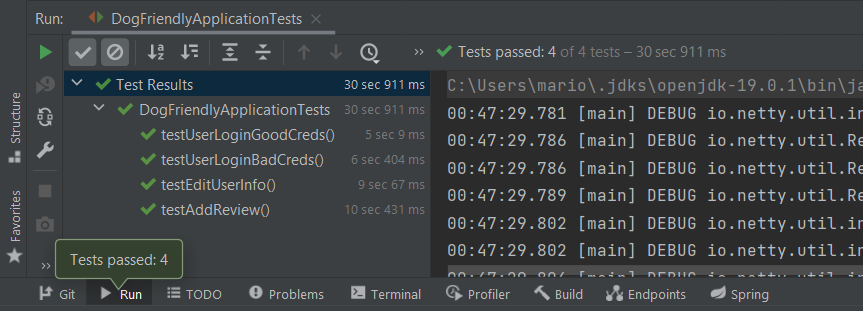
\includegraphics[width=\textwidth]{img/TestSuccess4.png}
        \centering
        \caption{Rezultati testova ispitivanja sustava}
    \end{figure}

    \eject
    \section{Dijagram razmještaja}

    Dijagram razmještaja prikazuje odnos programskih i sklopovskih dijelova te opisuje topologiju sustava. Klijent, koristeći HTTP protokol, preko klijentskog računala pristupa poslužiteljskom računalu. Poslužitelj koristi radni okvir Node.js preko kojeg se dohvaća stranica, Tomcat koji sadrži aplikaciju i funkcionalnosti te PostgreSql s bazom podataka.

    \begin{figure}[H]
        	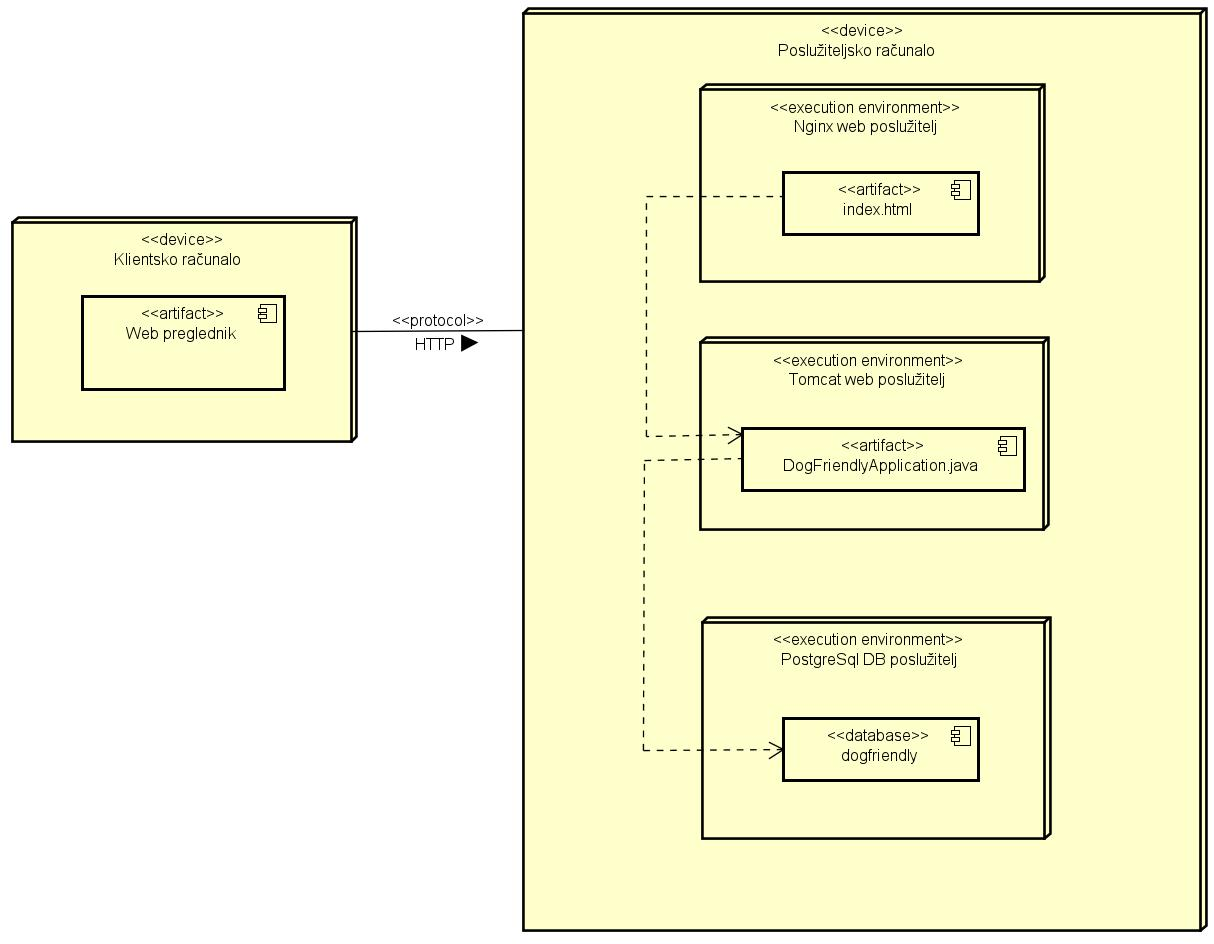
\includegraphics[width=\textwidth]{img/Dijagram_razmjestaja.jpg}
        	\centering
        	\caption{Dijagram razmještaja}
        	\label{fig:promjene}
        \end{figure}

    \eject
    \section{Upute za puštanje u pogon}

    Preduvjet za slijeđenje sljedećih uputa je instalirana instanca Ubuntu 22.04 operacijskog sustava na poslužitelju. Koraci u ovim uputama će gotovo sigurno raditi bez modifikacija na ostalim modernim inačicama Ubuntu operacijskog sustava, a uz manje modifikacije i na ostalim Linux operacijskim sustavima.

    \subsection{Konfiguracija baze podataka}

    Instalacija i pokretanje postgresql servisa
    \begin{lstlisting}[language=bash]
      sudo apt update
      sudo apt install postgresql postgresql-contrib
      sudo systemctl start postgresql.service
    \end{lstlisting}

    Zatim je potrebno konfigurirati vatrozid
    \begin{lstlisting}[language=bash]
      sudo ufw allow 5432
    \end{lstlisting}

    Sada se na sustav za upravljanje bazom podataka moguće spojiti pomoću alata PgAdmin. Potrebno je kliknuti na gumb "Add New Server" i zatim popuniti polja prikazana na slici.

    \begin{figure}[H]
    \centering
    \begin{subfigure}{.5\textwidth}
      \centering
      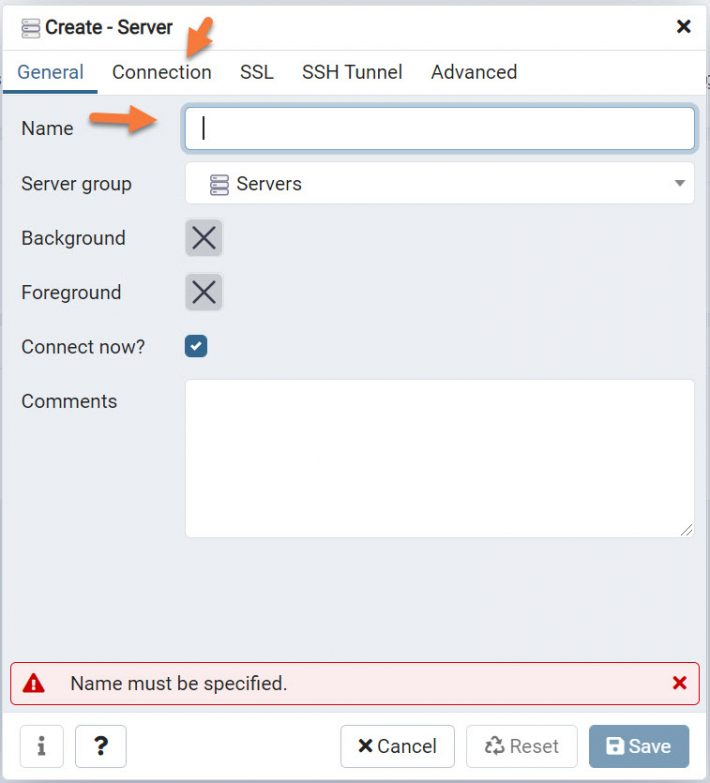
\includegraphics[width=0.9\linewidth]{img/2-1-710x783.jpg}
      \label{fig:sub1}
    \end{subfigure}%
    \begin{subfigure}{.5\textwidth}
      \centering
      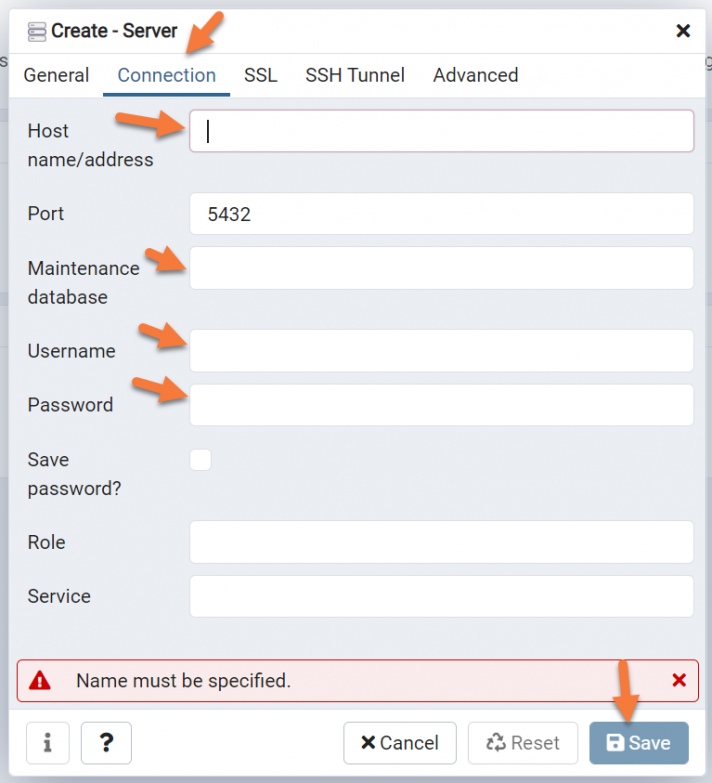
\includegraphics[width=0.9\linewidth]{img/115-712x783.png}
      \label{fig:sub2}
    \end{subfigure}
    \caption{Spajanje na sustav za upravljanje bazom podataka}
    \label{fig:test}
    \end{figure}

    Desnim klikom na upravo povezan poslužitelj, koji se nalazi u lijevoj traci alata, dolazimo do opcije "Create Database". Bazi podataka je potrebno dodijeliti ime i zatim je možemo pohraniti.
    Desnim klikom na novu bazu podataka dolazi se do opcije "Query Tool" koja otvara prozor s mogučnošću unosa nove SQL naredbe. Potrebno je kopirati sadržaj datoteke db.sql koja se nalazi unutar repozitorija te je zatim pokrenuti. Kopirane naredbe će stvoriti sve potrebne tablice, korisnike, uloge...

    \subsection{Backend poslužitelj}

    Prvi korak je izgradnja jar datoteke. Iz direktorija \textit{IzvorniKod/backend} potrebno je pokrenuti naredbu
    \begin{lstlisting}[language=bash]
      mvn package
    \end{lstlisting}
    Ako sve prođe po planu, generiranu jar datoteku koja se nalazi u target direktoriju, potrebno je kopirati na poslužitelj.
    Zatim je na poslužitelju potrebno stvoriti novi servis s putanjom \textit{/etc/systemd/system/dogfriendly-backend.service} i u njega staviti sljedeći kod
    \begin{lstlisting}[language=bash]
        [Unit]
        Description=Spring Boot backend for DogFriendly application
        After=network.target
        StartLimitIntervalSec=0
        
        [Service]
        Type=simple
        Restart=always
        RestartSec=1
        User=root
        ExecStart=/usr/bin/java -jar /home/leon3428/backend/DogFriendly-0.0.1-SNAPSHOT.jar
        
        [Install] 
        WantedBy=multi-user.target
    \end{lstlisting}
    
    Novonastali sevis tada možemo pokrenuti s
    \begin{lstlisting}[language=bash]
        sudo systemctl enable dogfiendly-backend.service
    \end{lstlisting}

    \eject
    \subsection{Frontend poslužitelj}

    Poslužitelj nginx instaliramo s
    \begin{lstlisting}[language=bash]
        sudo apt update
        sudo apt install nginx
    \end{lstlisting}
    Nakon što instalacija završi, potrebno je omogućiti port
    \begin{lstlisting}[language=bash]
        sudo ufw allow 'Nginx HTTP'
    \end{lstlisting}
    Sljedeći korak je konfiguracija bloka za dogfriendly domenu
    \begin{lstlisting}[language=bash]
        sudo mkdir -p /var/www/your_domain/html
        sudo chown -R $USER:$USER /var/www/your_domain/html
        sudo chmod -R 755 /var/www/your_domain
    \end{lstlisting}
    Potrebno je kopirati sljedeću konfiguraciju u datoteku \textit{/etc/nginx/sites-available/your\textunderscore domain}
    \begin{lstlisting}[language=bash]
        server {
                listen 80;
                listen [::]:80;
        
                root /var/www/dog-friendly.me/html;
                index index.html index.htm index.nginx-debian.html;
        
                server_name dog-friendly.me www.dog-friendly.me;
        	access_log  /var/log/nginx/access.log;
        	
        	location / {
            		try_files $uri /index.html;
        	}
        	location /api {  
          		proxy_pass http://localhost:5000;
          		proxy_http_version 1.1;
          		proxy_set_header Upgrade $http_upgrade;
          		proxy_set_header Connection 'upgrade';
          		proxy_set_header Host $host;
          		proxy_cache_bypass $http_upgrade; 
        	}
        }

    \end{lstlisting}
    Konfiguracijsku datoteku omogućimo s
    \begin{lstlisting}[language=bash]
        sudo ln -s /etc/nginx/sites-available/your_domain /etc/nginx/sites-enabled/
    \end{lstlisting}
    Poslužitelj bi sada trebao biti aktivan. Preostaje nam samo izgraditi React aplikaciju što možemo jednostavno napravit s naredbom
    \begin{lstlisting}[language=bash]
        npm run build
    \end{lstlisting}
    pozvanom iz direktorija \textit{IzvorniKod/frontend}.
    Sadržaj build direktorija je sada potrebno kopirati u direktorij \textit{/var/www/your\textunderscore domain/html} na poslužitelju.
    